\documentclass[pdftex, 11pt, a4paper, titlepage]{article}
\usepackage[slovak]{babel}
\usepackage[utf8]{inputenc}
\usepackage[IL2]{fontenc}
\usepackage[left=1.5cm, top=2.5cm, text={18cm, 25cm}]{geometry}
\usepackage{amsmath}
\usepackage{amsfonts}
\usepackage{graphicx}
\usepackage{pdfpages}
\usepackage{titlesec}   % For \titleformat
\usepackage{multirow}
\usepackage{float}
\usepackage{makecell}
%\usepackage{scalerel}

\graphicspath{ {./img/} }

% Set the section size to Huge, leave everything else same as the default defs
\titleformat{\section}
{\normalfont\Huge\bfseries}{\thesection}{1em}{}

\begin{document}
    \begin{titlepage}
        \begin{center}
            
\includegraphics[scale=0.15]{FIT_logo.png}\\[1.2cm]
            \Huge
            \textsc{\MakeUppercase{Vysoké učení technické v Brně}\\[0.5cm]
                    Fakulta informačních technologií}\\
            
            \vspace{\stretch{0.382}}
            \huge
            \textsc{\textbf{Projekt z MSP}}\\
            \vspace{\stretch{0.618}}
        \end{center}

        \LARGE
        % Putting this part into grouping parentheses {} just to be safe
        % that \noindent doesn't affect other text.
        {\noindent
        Spracoval: Patrik Németh\\
        Čísla zadaní: 19, 3\\
        Cvičenia -- skupina: streda, 10:00\\
        %TODO: toto \today vypise mesiac slovom.. mozno zmenit?
        \today\\}
    \end{titlepage}

    % The assignment text
    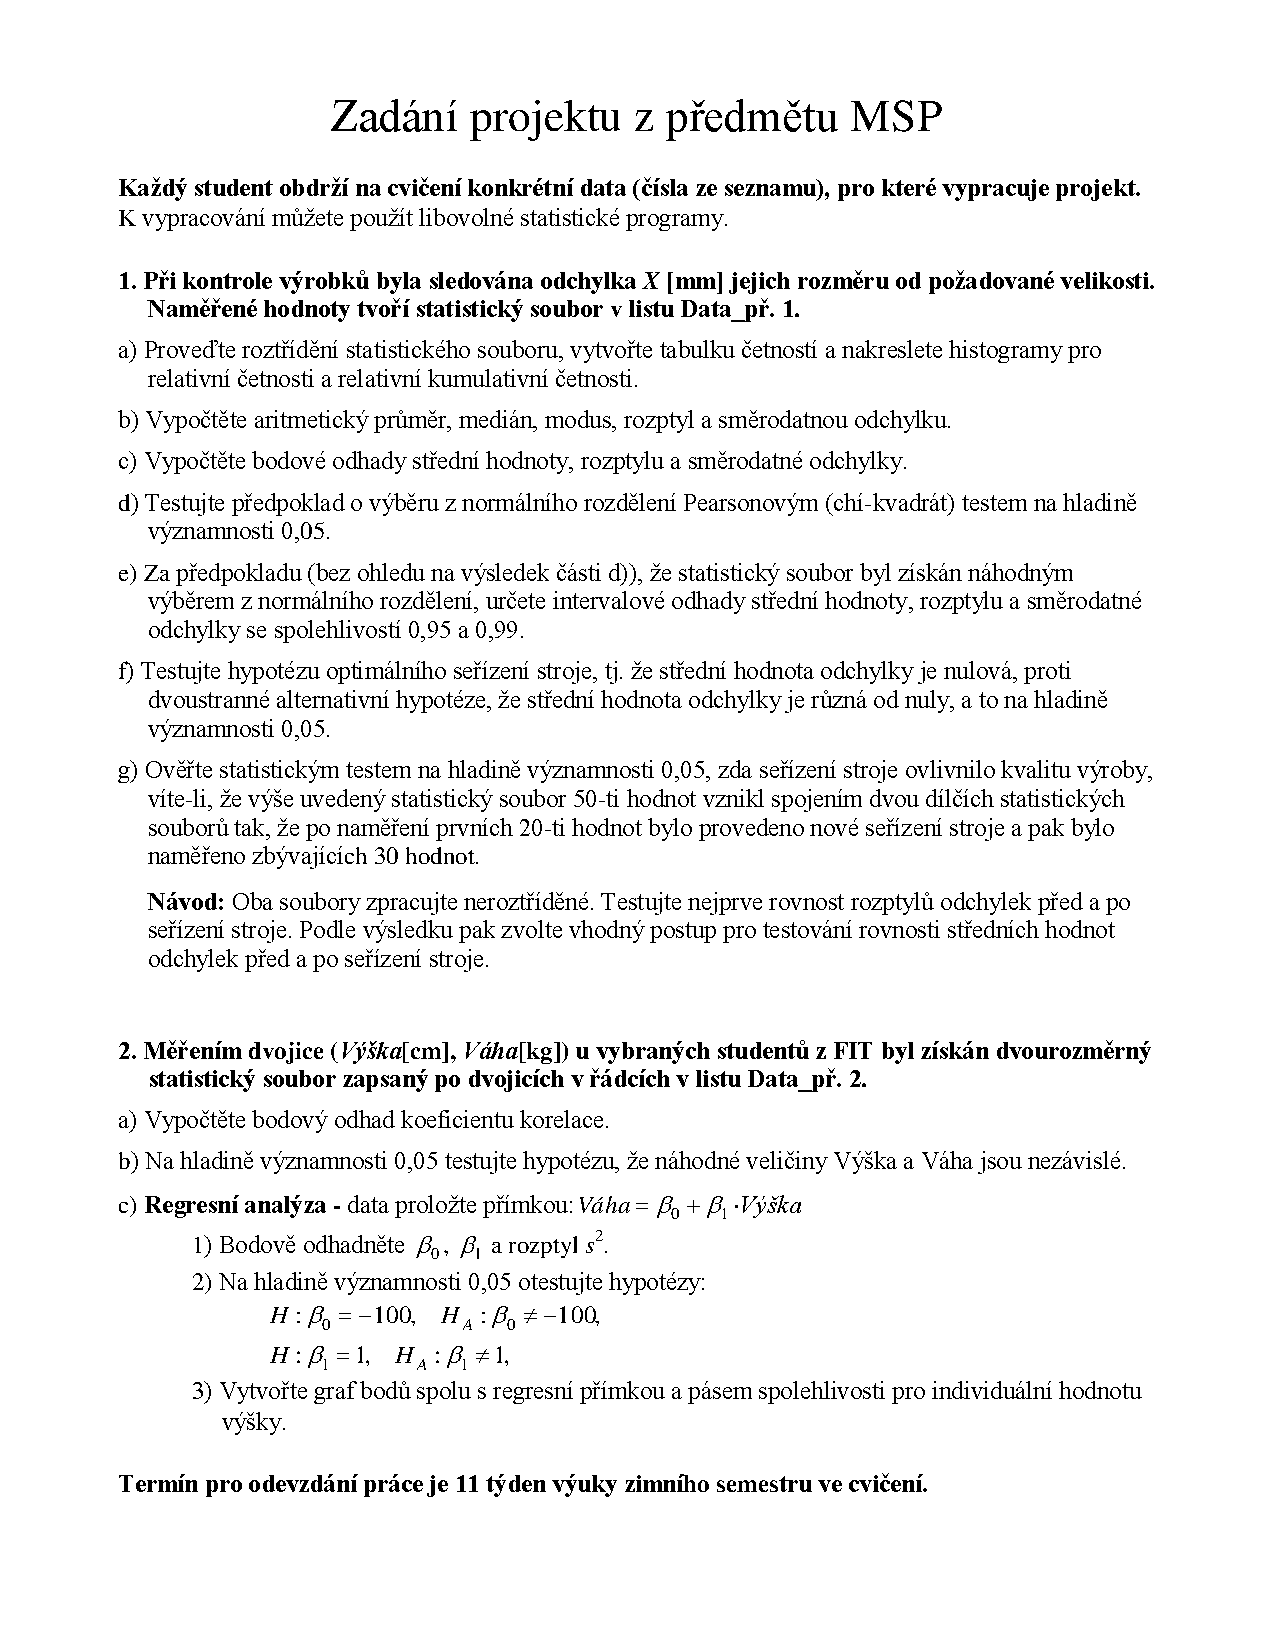
\includepdf[pages=-]{MSP_Projekt_2020-21_Zadani.pdf}

    \section*{Vypracovanie}


    \textbf{1. Při kontrole výrobků byla sledována odchylka $X$ [mm] jejich
    rozměru od požadované velikosti. Naměřené hodnoty tvoří statistický soubor
    v listu Data\_př. 1.}\\

    \begin{table}[H]
        % The minus '-' symbol was causing some issues, this is a fix from
        % https://www.abclinuxu.cz/tex/poradna/show/325037
        \catcode`\-=12
		\begin{tabular}{r|r|r|r|}
			\multicolumn{4}{r}{\thead{\textbf{Štatistický súbor}}} \\[1em]
			\cline{2-2} \cline{4-4}
			1 & $ 0,11 $ & 26 & $ 1,34 $ \\ \cline{2-2} \cline{4-4}
			2 & $ 1,17 $ & 27 & $ 1,94 $ \\ \cline{2-2} \cline{4-4}
			3 & $ 2,57 $ & 28 & $ 1,99 $ \\ \cline{2-2} \cline{4-4}
			4 & $ 1,77 $ & 29 & $ -0,32 $ \\ \cline{2-2} \cline{4-4}
			5 & $ 0,88 $ & 30 & $ 0,7 $ \\ \cline{2-2} \cline{4-4}
			6 & $ 1,45 $ & 31 & $ -0,35 $ \\ \cline{2-2} \cline{4-4}
			7 & $ 1,78 $ & 32 & $ 1,44 $ \\ \cline{2-2} \cline{4-4}
			8 & $ 1,56 $ & 33 & $ 1,63 $ \\ \cline{2-2} \cline{4-4}
			9 & $ 1,01 $ & 34 & $ -0,2 $ \\ \cline{2-2} \cline{4-4}
			10 & $ 2,25 $ & 35 & $ 0,87 $ \\ \cline{2-2} \cline{4-4}
			11 & $ 0,46 $ & 36 & $ -1,34 $ \\ \cline{2-2} \cline{4-4}
			12 & $ 0,23 $ & 37 & $ 2,07 $ \\ \cline{2-2} \cline{4-4}
			13 & $ 0,59 $ & 38 & $ -0,51 $ \\ \cline{2-2} \cline{4-4}
			14 & $ 0,92 $ & 39 & $ 3,31 $ \\ \cline{2-2} \cline{4-4}
			15 & $ 1,84 $ & 40 & $ 0,39 $ \\ \cline{2-2} \cline{4-4}
			16 & $ 2,26 $ & 41 & $ 1,38 $ \\ \cline{2-2} \cline{4-4}
			17 & $ -0,29 $ & 42 & $ -0,98 $ \\ \cline{2-2} \cline{4-4}
			18 & $ 2,06 $ & 43 & $ 0,53 $ \\ \cline{2-2} \cline{4-4}
			19 & $ 0,68 $ & 44 & $ -0,25 $ \\ \cline{2-2} \cline{4-4}
			20 & $ 2,1 $ & 45 & $ 0,59 $ \\ \cline{2-2} \cline{4-4}
			21 & $ 1,88 $ & 46 & $ 1,02 $ \\ \cline{2-2} \cline{4-4}
			22 & $ -0,01 $ & 47 & $ 1,36 $ \\ \cline{2-2} \cline{4-4}
			23 & $ 0,03 $ & 48 & $ 1,38 $ \\ \cline{2-2} \cline{4-4}
			24 & $ 0,36 $ & 49 & $ 1,98 $ \\ \cline{2-2} \cline{4-4}
			25 & $ 0,42 $ & 50 & $ -0,85 $ \\ \cline{2-2} \cline{4-4}
		\end{tabular}
%
		\hspace{4em}
%
        \begin{tabular}{r|r|r|r|}
            \multicolumn{4}{r}{\thead{\textbf{Usporiadaný štatistický súbor}}} \\[1em]
			\cline{2-2} \cline{4-4}
			(1) & $ -1.34 $ & (26) & $ 1.01 $ \\ \cline{2-2} \cline{4-4}
			(2) & $ -0.98 $ & (27) & $ 1.02 $ \\ \cline{2-2} \cline{4-4}
			(3) & $ -0.85 $ & (28) & $ 1.17 $ \\ \cline{2-2} \cline{4-4}
			(4) & $ -0.51 $ & (29) & $ 1.34 $ \\ \cline{2-2} \cline{4-4}
			(5) & $ -0.35 $ & (30) & $ 1.36 $ \\ \cline{2-2} \cline{4-4}
			(6) & $ -0.32 $ & (31) & $ 1.38 $ \\ \cline{2-2} \cline{4-4}
			(7) & $ -0.29 $ & (32) & $ 1.38 $ \\ \cline{2-2} \cline{4-4}
			(8) & $ -0.25 $ & (33) & $ 1.44 $ \\ \cline{2-2} \cline{4-4}
			(9) & $ -0.2 $ & (34) & $ 1.45 $ \\ \cline{2-2} \cline{4-4}
			(10) & $ -0.01 $ & (35) & $ 1.56 $ \\ \cline{2-2} \cline{4-4}
			(11) & $ 0.03 $ & (36) & $ 1.63 $ \\ \cline{2-2} \cline{4-4}
			(12) & $ 0.11 $ & (37) & $ 1.77 $ \\ \cline{2-2} \cline{4-4}
			(13) & $ 0.23 $ & (38) & $ 1.78 $ \\ \cline{2-2} \cline{4-4}
			(14) & $ 0.36 $ & (39) & $ 1.84 $ \\ \cline{2-2} \cline{4-4}
			(15) & $ 0.39 $ & (40) & $ 1.88 $ \\ \cline{2-2} \cline{4-4}
			(16) & $ 0.42 $ & (41) & $ 1.94 $ \\ \cline{2-2} \cline{4-4}
			(17) & $ 0.46 $ & (42) & $ 1.98 $ \\ \cline{2-2} \cline{4-4}
			(18) & $ 0.53 $ & (43) & $ 1.99 $ \\ \cline{2-2} \cline{4-4}
			(19) & $ 0.59 $ & (44) & $ 2.06 $ \\ \cline{2-2} \cline{4-4}
			(20) & $ 0.59 $ & (45) & $ 2.07 $ \\ \cline{2-2} \cline{4-4}
			(21) & $ 0.68 $ & (46) & $ 2.1 $ \\ \cline{2-2} \cline{4-4}
			(22) & $ 0.7 $ & (47) & $ 2.25 $ \\ \cline{2-2} \cline{4-4}
			(23) & $ 0.87 $ & (48) & $ 2.26 $ \\ \cline{2-2} \cline{4-4}
			(24) & $ 0.88 $ & (49) & $ 2.57 $ \\ \cline{2-2} \cline{4-4}
            (25) & $ 0.92 $ & (50) & $ 3.31 $ \\ \cline{2-2} \cline{4-4}
        \end{tabular}
    \end{table}

    \noindent\rule{\linewidth}{0.4pt}\\

    \noindent
    a) Proveďte roztřídění statistického souboru, vytvořte tabulku
    četností a nakreslete histogramy pro relativní četnosti a relativní
    kumulativní četnosti.\\
    
    \noindent
    $ x_{(1)} = \underset{i}{\text{min }}x_i = -1,34 $ \\
    $ x_{(n)} = \underset{i}{\text{max }}x_i = 3,31 $ \\
    Variačný obor: $ \langle{} x_{(1)}, x_{(n)} \rangle{} = \langle{} -1,34;3,31 \rangle{}$ \\
    Rozpätie: $ x_{(n)} - x_{(1)} = 4,65 $ \\
    Počet tried: $ m = 11 $ \\
    Dĺžka triedy: $ \dfrac{x_{(n)} - x_{(1)}}{m} = 0,4227272727 $ \\

    \begin{tabular}[]{|c|c|c|c|c|c|c|c|}
        \hline
        \textbf{trieda} & \textbf{x$_{i-}$} & \textbf{x$_{i+}$} & \textbf{stred triedy} & \textbf{kumul. poč.} & \textbf{poč.} & \textbf{relat. poč.} & \textbf{relat. kumul. poč.} \\
        \hline
        1   &   $-1,3400$ & $-0,9173$   &   $-1,1286$ & $2$ &   $2$ & $0,04$ &  $0,04$ \\
        2   &   $-0,9173$ & $-0,4945$   &   $-0,7059$ & $4$ &   $2$ & $0,04$ &  $0,08$ \\
        3   &   $-0,4945$ & $-0,0718$   &   $-0,2832$ & $9$ &   $5$ & $0,1$ &   $0,18$ \\
        4   &   $-0,0718$ & $0,3509$    &   $0,1395$ &  $13$ &  $4$ & $0,08$ &  $0,26$ \\
        5   &   $0,3509$  & $0,7736$   &    $0,5623$ &   $22$ &  $9$ & $0,18$ &  $0,44$ \\
        6   &   $0,7736$  & $1,1964$   &    $0,9850$ &   $28$ &  $6$ & $0,12$ &  $0,56$ \\
        7   &   $1,1964$  & $1,6191$   &    $1,4077$ &   $35$ &  $7$ & $0,14$ &  $0,7$ \\
        8   &   $1,6191$  & $2,0418$   &    $1,8305$ &   $43$ &  $8$ & $0,16$ &  $0,86$ \\
        9   &   $2,0418$  & $2,4645$   &    $2,2532$ &   $48$ &  $5$ & $0,1$ &   $0,96$ \\
        10  &   $2,4645$   & $2,8873$   &   $2,6759$ &   $49$ &  $1$ & $0,02$ &  $0,98$ \\
        11  &   $2,8873$   & $3,3100$   &   $3,0986$ &   $50$ &  $1$ & $0,02$ &  $1$ \\
        \hline
    \end{tabular}

    \begin{center}
        \noindent
        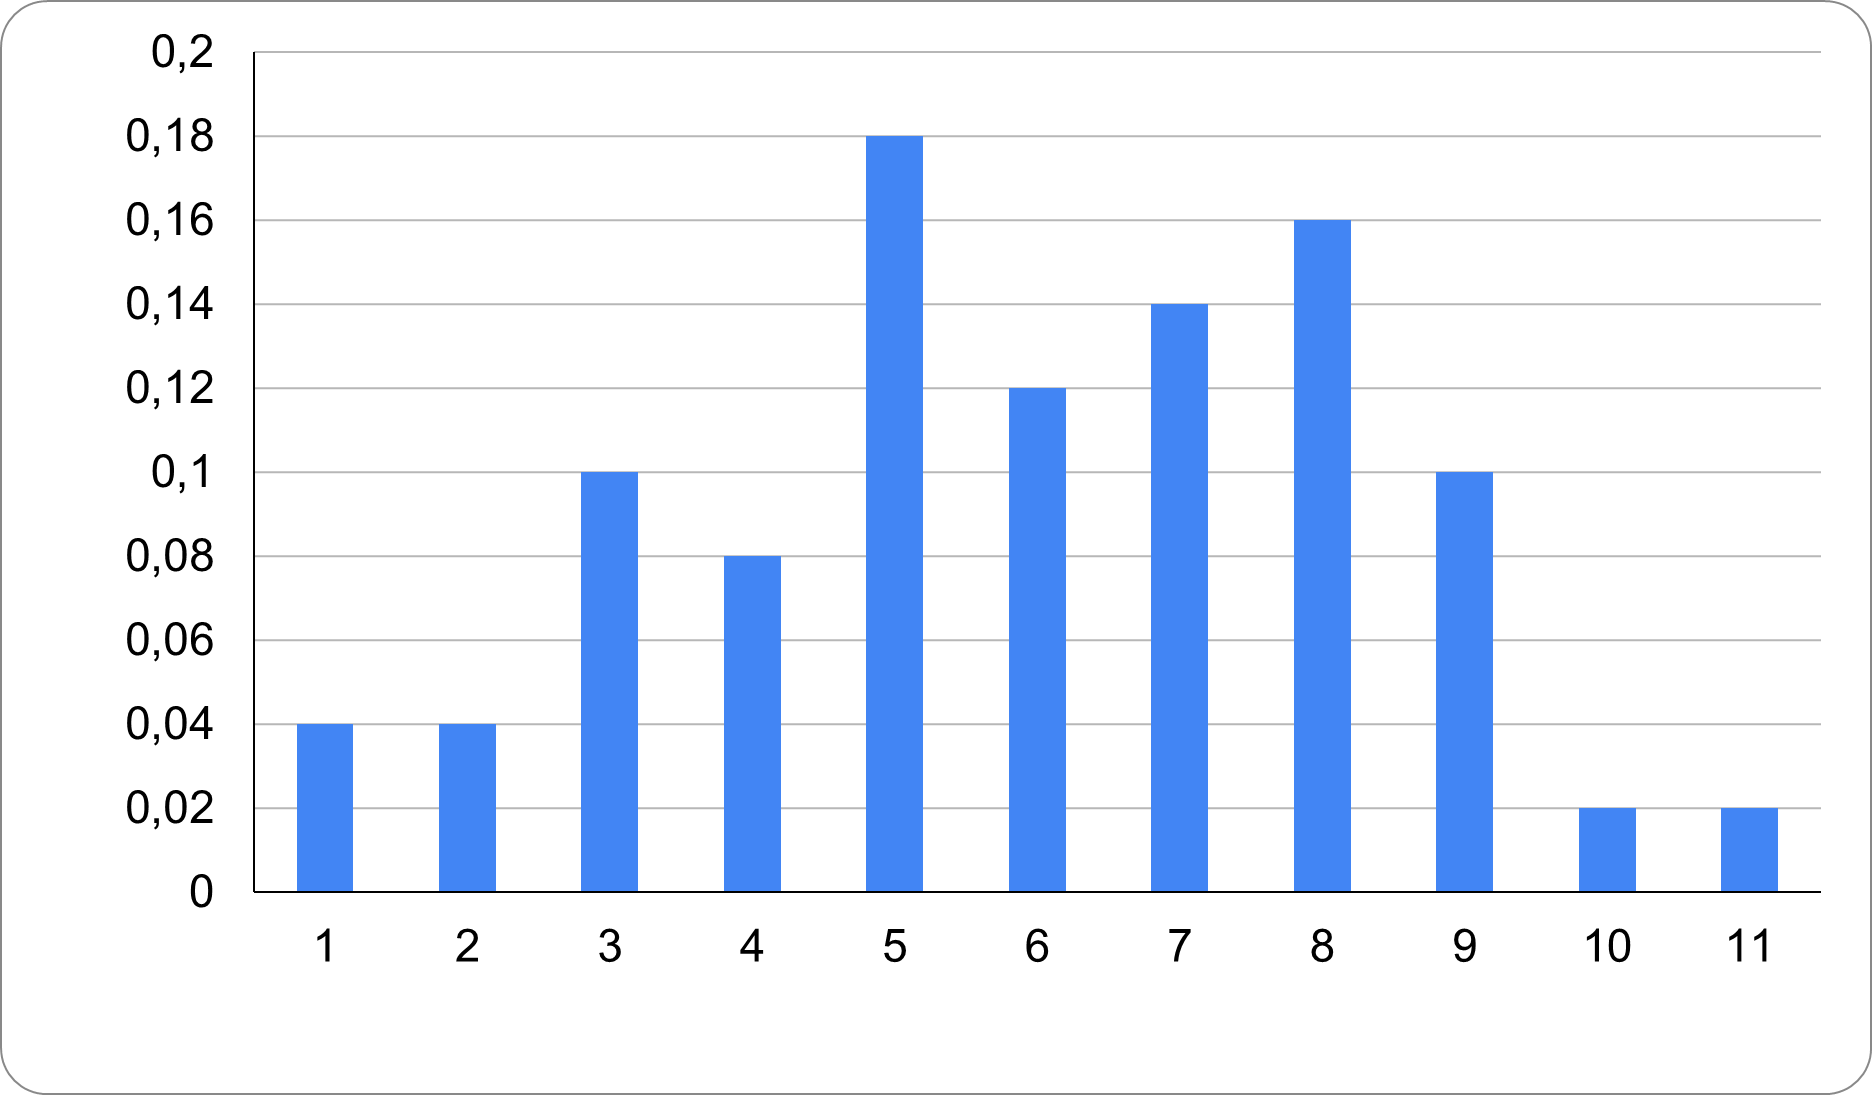
\includegraphics[scale=0.8]{histogram_relat_pocetnost.png}\\\vspace{5pt}
        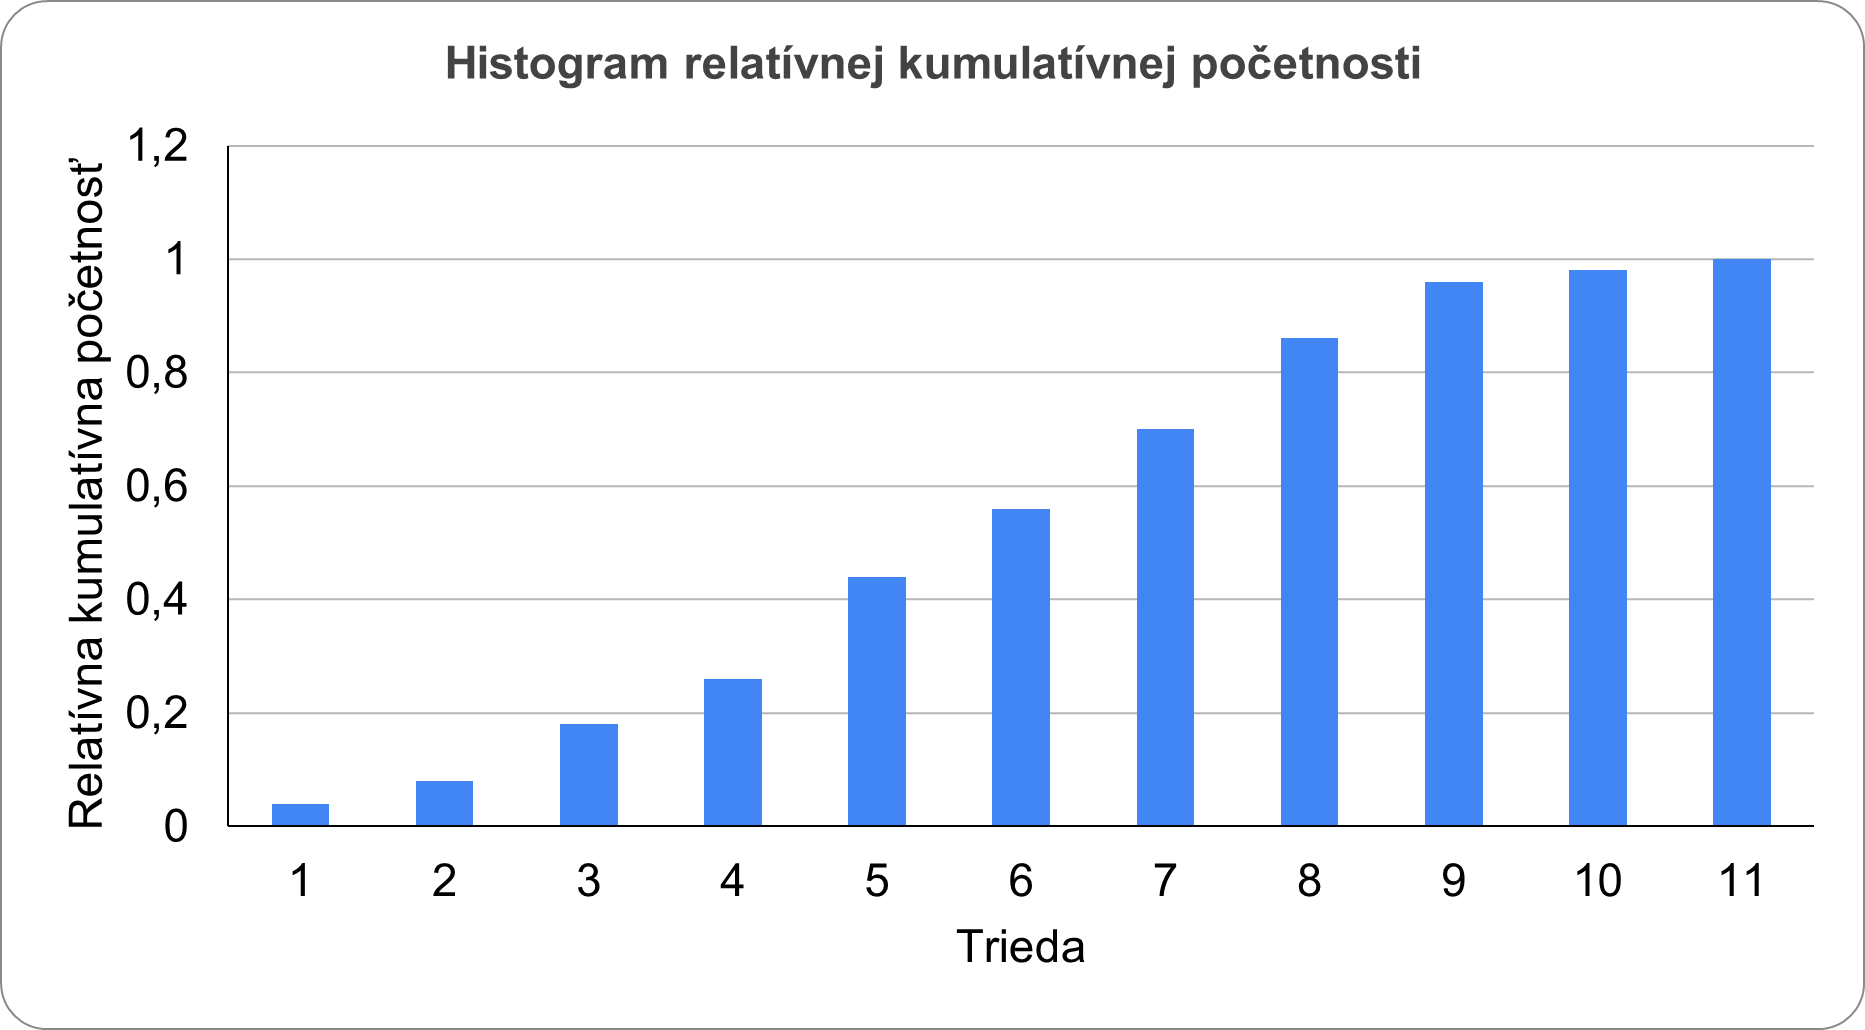
\includegraphics[scale=0.8]{histogram_relat_kumul_pocetnost.png}
    \end{center}

    \noindent\rule{\linewidth}{0.4pt}\\

    \noindent
    b) Vypočtěte aritmetický průměr, medián, modus, rozptyl a směrodatnou
    odchylku.

    \noindent
    $ \overline{x} = \dfrac{1}{n} \sum\limits_{i=1}^{n} x_i = 0,944 $ \\
    Medián: $ \tilde{x} = 0,965 $ \\
    Modus: $ \hat{x} = 0,562272 $ \\
    $ s^2 = \dfrac{1}{n} \sum\limits_{i=1}^{n} (x_i - \overline{x})^2 = 1,006424 $ \\
    $ s = \sqrt{\dfrac{1}{n} \sum\limits_{i=1}^{n} (x_i - \overline{x})^2} = 1,003206 $ \\

    \noindent\rule{\linewidth}{0.4pt}\\

    \noindent
    c) Vypočtěte bodové odhady střední hodnoty, rozptylu a směrodatné odchylky.

    \noindent
    Bodový odhad strednej hodnoty: $ \overline{x} = \dfrac{1}{n} \sum\limits_{i=1}^{n} x_i = 0,944 $ \\
    \noindent
    Bodový odhad rozptylu: $ s^2 = \dfrac{1}{n-1} \sum\limits_{i=1}^{n} (x_i - \overline{x})^2 = 1,026963 $ \\
    \noindent
    Bodový odhad smerodatnej odchýľky: $ s = \sqrt{\dfrac{1}{n-1} \sum\limits_{i=1}^{n} (x_i - \overline{x})^2} = 1,013391 $ \\
    
    \noindent\rule{\linewidth}{0.4pt}\\

    \noindent
    d) Testujte předpoklad o výběru z normálního rozdělení Pearsonovým
    (chí-kvadrát) testem na hladině významnosti 0,05.\\

    \begin{tabular}[]{|c|c|c|c|c|c|c|c|}
        \hline
        \textbf{trieda} & \textbf{x$_{i-}$} & \textbf{x$_{i+}$} & \textbf{stred triedy} & \textbf{kumul. poč.} & \textbf{poč.} & \textbf{teor. poč.} & $\dfrac{\text{\textbf{rozdiel}}^2}{\text{\textbf{teor. poč.}}}$ \\
        \hline
        1   &   $-1000$     & $-0,0718$ & $-500,0359$   & $9$   & $9$ & $7,9038$ & $0,1520$ \\
        2   &   $-0,0718$   & $0,3509$  & $0,1395$      & $13$  & $4$ & $6,0556$ & $0,6978$ \\
        3   &   $0,3509$    & $0,7736$  & $0,5623$      & $22$  & $9$ & $7,7029$ & $0,2184$ \\
        4   &   $0,7736$    & $1,1964$  & $0,9850$      & $28$  & $6$ & $8,2542$ & $0,6156$ \\
        5   &   $1,1964$    & $1,6191$  & $1,4077$      & $35$  & $7$ & $7,4509$ & $0,0273$ \\
        6   &   $1,6191$    & $2,0418$  & $1,8305$      & $43$  & $8$ & $5,6658$ & $0,9616$ \\
        7   &   $2,0418$    & $1000$    & $501,0209$    & $50$  & $7$ & $6,9668$ & $0,0002$ \\
        \hline
    \end{tabular}

    \noindent
    Testovacie kritérium: $ t= \sum\limits_{j=1}^{m} \dfrac{(f_j - \hat{f}_j)^2}{\hat{f}_j} = 2,6727$,\\

    \noindent
    $ \chi{}_{1-\alpha}^2 $ pre $ k = 7-2-1 $ stupňov voľnosti: $ 9,4877 $,\\

    \noindent
    doplnok kritického oboru: $ \overline{W_\alpha} = \langle 0;\chi{}_{1-\alpha}^2 \rangle = \langle 0;9,4877 \rangle $.\\

    \noindent
    Keďže $ t \in \overline{W_\alpha} $, tak sa hypotéza $ X \sim N(0,944; 1,027) $ \textbf{nezamieta}.

    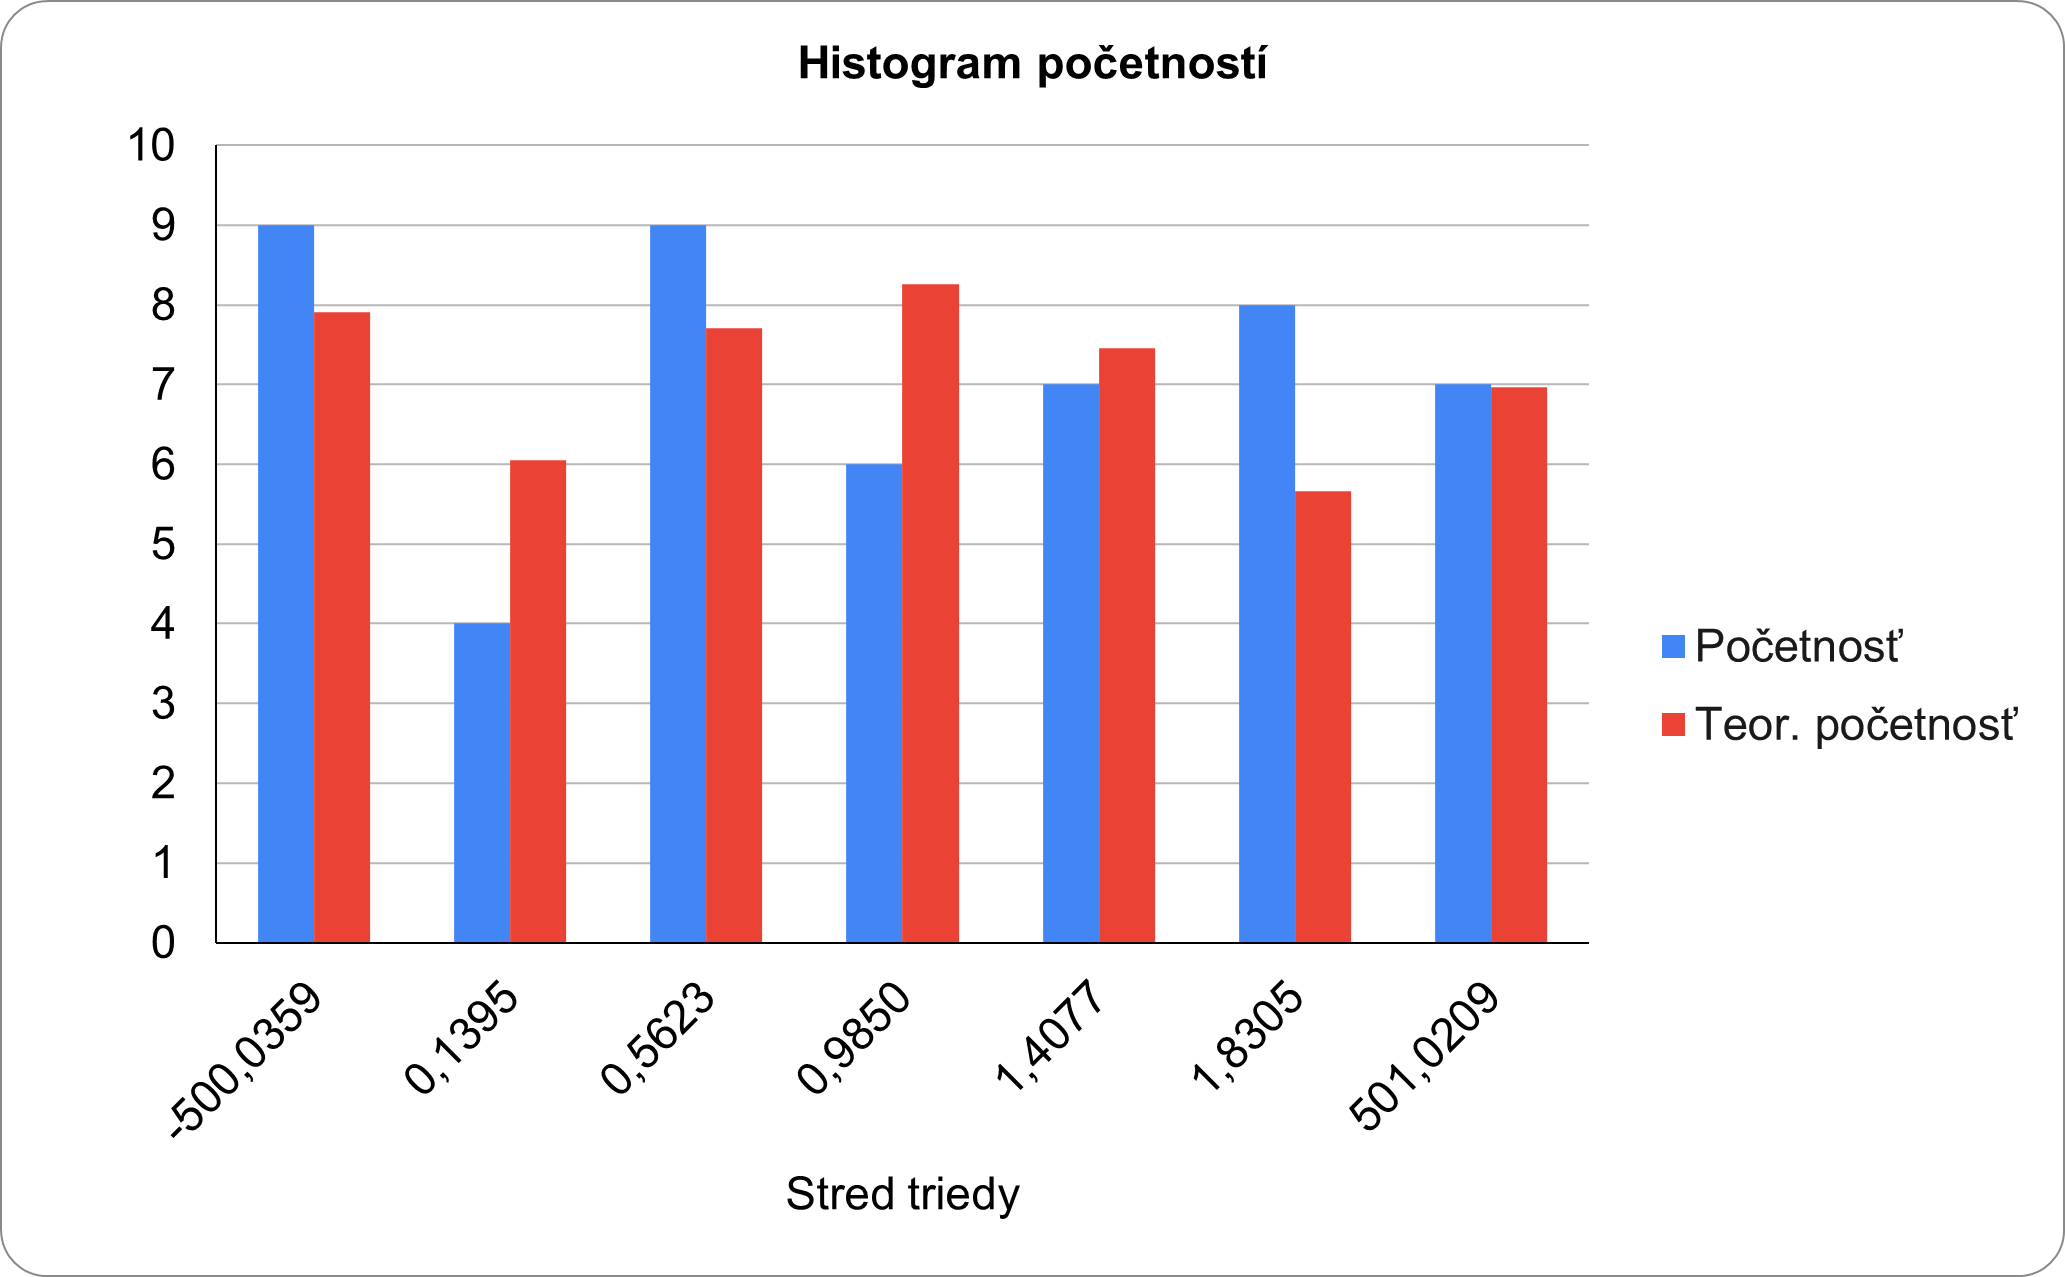
\includegraphics[scale=0.8]{histogram_pocetnosti.png}

    \newpage
    \noindent\rule{\linewidth}{0.4pt}\\

    \noindent
    e) Za předpokladu (bez ohledu na výsledek části d)), že statistický soubor
    byl získán náhodným výběrem z normálního rozdělení, určete intervalové odhady
    střední hodnoty, rozptylu a směrodatné odchylky se spolehlivostí 0,95 a 0,99.\\

    \noindent
    Predpoklad: $ X \sim N(\mu,\sigma^2), \mu $ a $ \sigma^2 $ sú neznáme.\\

    \noindent
    Bodový odhad strednej hodnoty: $ \overline{x} = \dfrac{1}{n} \sum\limits_{i=1}^{n} x_i = 0,944 $ \\
    Bodový odhad rozptylu: $ s^2 = \dfrac{1}{n-1} \sum\limits_{i=1}^{n} (x_i - \overline{x})^2 = 1,026963 $ \\
    Bodový odhad smerodatnej odchýľky: $ s = \sqrt{\dfrac{1}{n-1} \sum\limits_{i=1}^{n} (x_i - \overline{x})^2} = 1,013391 $ \\

    \noindent
    \textbf{Intervalový odhad parametru $\mu$:}\\
    0,975 kvantil Študentovho rozdelenia $t_{1-\alpha/2}$ s $k=n-1=50-1=49$
    stupňami voľnosti $=2,009575237$\\
    0,995 kvantil Študentovho rozdelenia $t_{1-\alpha/2}$ s $k=n-1=50-1=49$
    stupňami voľnosti $=2,679951974$\\

    \noindent
    $\alpha=0,05:\left\langle \overline{x}-t_{1-\alpha/2}\dfrac{s}{\sqrt{n}} ; \overline{x}+t_{1-\alpha/2}\dfrac{s}{\sqrt{n}} \right\rangle = \langle 0,655997191483301 ; 1,2320028085167 \rangle$\\
    $\alpha=0,01:\left\langle \overline{x}-t_{1-\alpha/2}\dfrac{s}{\sqrt{n}} ; \overline{x}+t_{1-\alpha/2}\dfrac{s}{\sqrt{n}} \right\rangle = \langle 0,559921971551384 ; 1,32807802844862 \rangle$\\


    \noindent
    \textbf{Intervalový odhad parametru $\sigma^2$:}\\
    \noindent
    0,975 kvantil Pearsonovho rozdelenia $\chi_{\alpha/2}^{2}$ s $k = n-1 = 50-1=49$
    stupňami voľnosti $=31,5549164626671$\\
    0,975 kvantil Pearsonovho rozdelenia $\chi_{1-\alpha/2}^{2}$ s $k = n-1 = 50-1=49$
    stupňami voľnosti $=70,2224135664345$\\
    0,995 kvantil Pearsonovho rozdelenia $\chi_{\alpha/2}^{2}$ s $k = n-1 = 50-1=49$
    stupňami voľnosti $=27,2493490695696$\\
    0,995 kvantil Pearsonovho rozdelenia $\chi_{1-\alpha/2}^{2}$ s $k = n-1 = 50-1=49$
    stupňami voľnosti $=78,2307080866899$\\

    \noindent
    $\alpha=0,05: \left\langle \dfrac{(n-1)s^2}{\chi_{1-\alpha/2}^2} ; \dfrac{(n-1)s^2}{\chi_{\alpha/2}^2} \right\rangle = \langle 0,716597414476408 ; 1,59471821323106 \rangle$\\
    $\alpha=0,01: \left\langle \dfrac{(n-1)s^2}{\chi_{1-\alpha/2}^2} ; \dfrac{(n-1)s^2}{\chi_{\alpha/2}^2} \right\rangle = \langle 0,643241014055983 ; 1,84669365391174 \rangle$\\

    \noindent
    \textbf{Intervalový odhad parametru $\sigma$:}\\

    \noindent
    $\alpha=0,05: \left\langle \sqrt{\dfrac{(n-1)s^2}{\chi_{1-\alpha/2}^2}} ; \sqrt{\dfrac{(n-1)s^2}{\chi_{\alpha/2}^2}} \right\rangle = \langle 0,846520770256943 ; 1,26282152865362 \rangle$\\
    $\alpha=0,01: \left\langle \sqrt{\dfrac{(n-1)s^2}{\chi_{1-\alpha/2}^2}} ; \sqrt{\dfrac{(n-1)s^2}{\chi_{\alpha/2}^2}} \right\rangle = \langle 0,802023075762775 ; 1,35893107033129 \rangle$\\

    \noindent\rule{\linewidth}{0.4pt}\\

    \noindent
    f) Testujte hypotézu optimálního seřízení stroje, tj. že střední hodnota
    odchylky je nulová, proti dvoustranné alternativní hypotéze, že střední
    hodnota odchylky je různá od nuly, a to na hladině významnosti 0,05.\\

    \noindent
    \textbf{Študentov jednovýberový test:}\\
    \noindent
    Testujeme \textbf{hypotézu} $H_0:\mu = 0$ oproti \textbf{alternatívnej hypotéze} $H_A:\mu \neq 0$:\\

    \noindent
    testovacie kritérium: $t = \dfrac{\overline{x}-\mu_0}{s} \sqrt{n} = \dfrac{\overline{x}-0}{s} \sqrt{n} = 6,58687682116824$\\
    
    \noindent
    doplnok kritického oboru: $\overline{W_\alpha} = \left\langle -t_{1-\alpha/2}, t_{1-\alpha/2} \right\rangle$ pre alternatívnu hypotézu $H_A$,\\
    $0,975$ kvantil Študentovho rozdelenia $t_{1-\alpha/2}$ s $k=n-1=50-1=49$ stupňami voľnosti $=2,00957523712924$\\
    $\overline{W_\alpha} = \left\langle -t_{1-\alpha/2}, t_{1-\alpha/2} \right\rangle = \left\langle -2,00957523712924 ; 2,00957523712924\right\rangle$\\

    \noindent
    Keďže $t \notin \overline{W_\alpha}$, tak sa hypotéza $H_0 : \mu = 0$ \textbf{zamieta} a alternatívna hypotéza $H_A:\mu \neq 0$ \textbf{nezamieta}.\\

    \noindent\rule{\linewidth}{0.4pt}\\
    g) Ověřte statistickým testem na hladině významnosti 0,05, zda seřízení
    stroje ovlivnilo kvalitu výroby, víte-li, že výše uvedený statistický soubor
    50-ti hodnot vznikl spojením dvou dílčích statistických souborů tak,
    že po naměření prvních 20-ti hodnot bylo provedeno nové seřízení stroje
    a pak bylo naměřeno zbývajících 30 hodnot.\\

    \noindent
    \begin{table}[H]
        \catcode`\-=12
		\begin{tabular}[t]{r|r|}
			\multicolumn{1}{c}{} & \multicolumn{1}{c}{$ \boldsymbol{x\ 1:20}
			$\,--\,$\boldsymbol{X} $} \\ \cline{2-2}

			1 & $ 0.11 $ \\ \cline{2-2}
			2 & $ 1.17 $ \\ \cline{2-2}
			3 & $ 2.57 $ \\ \cline{2-2}
			4 & $ 1.77 $ \\ \cline{2-2}
			5 & $ 0.88 $ \\ \cline{2-2}
			6 & $ 1.45 $ \\ \cline{2-2}
			7 & $ 1.78 $ \\ \cline{2-2}
			8 & $ 1.56 $ \\ \cline{2-2}
			9 & $ 1.01 $ \\ \cline{2-2}
			10 & $ 2.25 $ \\ \cline{2-2}
			11 & $ 0.46 $ \\ \cline{2-2}
			12 & $ 0.23 $ \\ \cline{2-2}
			13 & $ 0.59 $ \\ \cline{2-2}
			14 & $ 0.92 $ \\ \cline{2-2}
			15 & $ 1.84 $ \\ \cline{2-2}
			16 & $ 2.26 $ \\ \cline{2-2}
			17 & $ -0.29 $ \\ \cline{2-2}
			18 & $ 2.06 $ \\ \cline{2-2}
			19 & $ 0.68 $\\ \cline{2-2}
			20 & $ 2.1 $ \\ \cline{2-2}
		\end{tabular}
%
		\hspace{4em}
%
		\begin{tabular}[t]{r|r|}
			\multicolumn{1}{c}{} & \multicolumn{1}{c}{$ \boldsymbol{x\ 21:50}
			$\,--\,$ \boldsymbol{Y} $} \\ \cline{2-2}

			21 & $ 1.88 $ \\ \cline{2-2}
			22 & $ -0.01 $ \\ \cline{2-2}
			23 & $ 0.03 $ \\ \cline{2-2}
			24 & $ 0.36 $ \\ \cline{2-2}
			25 & $ 0.42 $ \\ \cline{2-2}
			26 & $ 1.34 $ \\ \cline{2-2}
			27 & $ 1.94 $ \\ \cline{2-2}
			28 & $ 1.99 $ \\ \cline{2-2}
			29 & $ -0.32 $ \\ \cline{2-2}
			30 & $ 0.7 $ \\ \cline{2-2}
			31 & $ -0.35 $ \\ \cline{2-2}
			32 & $ 1.44 $ \\ \cline{2-2}
			33 & $ 1.63 $ \\ \cline{2-2}
			34 & $ -0.2 $ \\ \cline{2-2}
			35 & $ 0.87 $ \\ \cline{2-2}
			36 & $ -1.34 $ \\ \cline{2-2}
			37 & $ 2.07 $ \\ \cline{2-2}
			38 & $ -0.51 $ \\ \cline{2-2}
			39 & $ 3.31 $ \\ \cline{2-2}
			40 & $ 0.39 $ \\ \cline{2-2}
			41 & $ 1.38 $ \\ \cline{2-2}
			42 & $ -0.98 $ \\ \cline{2-2}
			43 & $ 0.53 $ \\ \cline{2-2}
			44 & $ -0.25 $ \\ \cline{2-2}
			45 & $ 0.59 $ \\ \cline{2-2}
			46 & $ 1.02 $ \\ \cline{2-2}
			47 & $ 1.36 $ \\ \cline{2-2}
			48 & $ 1.38 $ \\ \cline{2-2}
			49 & $ 1.98 $ \\ \cline{2-2}
			50 & $ -0.85 $ \\ \cline{2-2}
		\end{tabular}
	\end{table}

    \begin{table}[H]
        \catcode`\-=12
        \begin{tabular}{l|r|r|}
            \cline{2-3}
            & $ \boldsymbol{X} $ & $ \boldsymbol{Y} $ \\
            \cline{2-3}
			\textbf{počet} $ \boldsymbol{n} $ & $ 20 $ & $ 30 $ \\
			\textbf{priemer} $ \boldsymbol{\overline{x}} $ & $ 1,27 $
			& $ 0,726667 $ \\

			\textbf{bodový odhad rozptylu} $ \boldsymbol{s^2} $ & $ 0,661821 $
			& $ 1,179451 $ \\

			\textbf{bodový odhad smerodatnej odchýľky} $ \boldsymbol{s} $ & $ 0,813524 $
            & $ 1,086025 $ \\
            \cline{2-3}
		\end{tabular}
    \end{table}

    \newpage
    \noindent
    \textbf{Test rovnosti rozptylov:}\\
    \textbf{Testuje sa hypotéza} $H_0 : \sigma_X^2 = \sigma_Y^2$:\\

    \noindent
    testovacie kritérium: $t = \dfrac{s^2(X)}{s^2(Y)} = \dfrac{0,661821}{1,179451} = 0,561127$\\
    doplnok kritického oboru: $\overline{W_\alpha} = \left\langle F_{\alpha/2}(n-1,m-1), F_{1-\alpha/2}(n-1,m-1) \right\rangle$ pre $H_A : \sigma_X^2 \neq \sigma_Y^2$,\\
    $F_{\alpha/2}(k_1,k_2), F_{1-\alpha/2}(k_1,k_2)$ sú kvantily Fischer-Snedecerovho rozdelenia s $k_1 = n-1$ a $k_2 = m-1$ stupňami voľnosti.\\
    $F_{\alpha/2}(19,29) = 0,41632$\\
    $F_{1-\alpha/2}(19,29) = 2,231274$\\
    $\left\langle F_{\alpha/2}(n-1,m-1), F_{1-\alpha/2}(n-1,m-1) \right\rangle = \left\langle 0,41632 ; 2,231274 \right\rangle$\\
    Keďže $t \in \overline{W_\alpha}$, tak sa hypotéza $H_0 : \sigma_X^2 = \sigma_Y^2$ \textbf{nezamieta}.\\

    \noindent
    \textbf{Študentov dvojvýberový test:}\\
    \textbf{Testuje sa hypotéza} $H_0 : \mu_X - \mu_Y = 0$ \textbf{za podmienky} $\sigma_X^2 = \sigma_Y^2$\\

    \noindent
    testovacie kritérium: $t = \dfrac{\overline{x}-\overline{y}-\mu_0}{\sqrt{(n-1)s^2(X)+(m-1)s^2(Y)}}\sqrt{\dfrac{nm(n+m-2)}{n+m}} = 1,906574$\\
    doplnok kritického oboru: $\overline{W_\alpha} = \left\langle -t_{1-\alpha/2}, t_{1-\alpha/2} \right\rangle$ pre $H_A : \mu_X - \mu_Y \neq 0$,\\
    $t_{1-\alpha/2}$ - kvantil Študentovho rozdelenia s $k=n+m-2=20+30-2=48$ stupňami voľnosti.\\
    $t_{1-\alpha/2} = 2,010635$\\
    $\overline{W_\alpha} = \left\langle -t_{1-\alpha/2}, t_{1-\alpha/2} \right\rangle = \left\langle -2,010635 ; 2,010635 \right\rangle$\\
    Keďže $t \in \overline{W_\alpha}$, tak sa hypotéza $H_0 : \mu_X - \mu_Y = 0$ \textbf{nezamieta}.

    % TASK 2
    \newpage
    \noindent
    \textbf{2. Měřením dvojice (\emph{Výška}[cm], \emph{Váha}[kg]) u vybraných studentů
    z FIT byl získán dvourozměrný statistický soubor zapsaný po dvojicích
    v řádcích v listu Data\_př. 2.}\\

    \begin{table}[H]
		\begin{tabular}{|r|r|}
			\multicolumn{1}{c}{\textbf{$ \boldsymbol{X} $\,--\,Výška [cm]}}
			& \multicolumn{1}{c}{\textbf{$ \boldsymbol{Y} $\,--\,Váha [kg]}}
			\\ \hline

			$ 166 $ & $ 67 $ \\ \hline
			$ 152 $ & $ 52 $ \\ \hline
			$ 154 $ & $ 78 $ \\ \hline
			$ 155 $ & $ 57 $ \\ \hline
			$ 190 $ & $ 109 $ \\ \hline
			$ 182 $ & $ 97 $ \\ \hline
			$ 153 $ & $ 58 $ \\ \hline
			$ 193 $ & $ 95 $ \\ \hline
			$ 191 $ & $ 98 $ \\ \hline
			$ 166 $ & $ 82 $ \\ \hline
			$ 164 $ & $ 68 $ \\ \hline
			$ 186 $ & $ 90 $ \\ \hline
			$ 175 $ & $ 85 $ \\ \hline
			$ 154 $ & $ 54 $ \\ \hline
			$ 200 $ & $ 104 $ \\ \hline
			$ 199 $ & $ 110 $ \\ \hline
			$ 164 $ & $ 75 $ \\ \hline
			$ 200 $ & $ 119 $ \\ \hline
			$ 180 $ & $ 94 $ \\ \hline
			$ 158 $ & $ 65 $ \\ \hline
		\end{tabular}
    \end{table}
    
    \noindent
    $n = 20$\\
    $\overline{x} = 174,1$\\
    $\overline{y} = 82,85$\\
    $\sum\limits_{i=1}^{n}x_i^2 = 612014$\\
    $\sum\limits_{i=1}^{n}y_i^2 = 145161$\\
    $\sum\limits_{i=1}^{n}x_iy_i = 294839$\\

    \noindent\rule{\linewidth}{0.4pt}\\

    \noindent
    a) Vypočtěte bodový odhad koeficientu korelace.\\
    
    \noindent
    $r = \dfrac{\sum\limits_{i=1}^{n}x_iy_i - n\overline{x}\overline{y}}{\sqrt{\left( \sum\limits_{i=1}^{n}x_i^2 - n\overline{x}^2 \right) \left( \sum\limits_{i=1}^{n}y_i^2 - n\overline{y}^2 \right)}} = 0,940332$\\

    \noindent\rule{\linewidth}{0.4pt}\\

    \noindent
    b) Na hladině významnosti 0,05 testujte hypotézu, že náhodné veličiny
    Výška a Váha jsou nezávislé.\\

    \noindent
    Testuje sa hypotéza $H_0 : \rho = 0$:\\
    testovacie kritérium: $t = \dfrac{|r|\sqrt{n-2}}{\sqrt{1-r^2}} = 11,724906$\\
    doplnok kritického oboru: $\overline{W_\alpha} = \left\langle 0,t_{1-\alpha/2} \right\rangle$ pre alternatívnu hypotézu: $H_A: \rho \neq 0$,\\
    $t_{1-\alpha/2}(n-2) = 2,100922$, čím $\overline{W_\alpha} = \left\langle 0;2,100922 \right\rangle$\\
    Keďže $t \notin \overline{W_\alpha}$, tak sa hypotéza $H_0 : \rho = 0$ sa \textbf{zamieta}.\\

    \noindent\rule{\linewidth}{0.4pt}\\

    \noindent
    c) \textbf{Regresní analýza} - data proložte přímkou: $\text{\emph{Váha}} = \beta_0 + \beta_1\cdot\text{\emph{Výška}}$
    \begin{enumerate}
        \item Bodově odhadněte $\beta_0$, $\beta_1$ a rozptyl $s^2$.
        \item Na hladině významnosti $0,05$ otestujte hypotézy:\\
            $H : \beta_0 = -100$, $H_A : \beta_0 \neq -100$,\\
            $H : \beta_1 = 1$, $H_A : \beta_1 \neq 1$,
        \item Vytvořte graf bodů spolu s regresní přímkou a pásem spolehlivosti pro individuální hodnotu výšky.\\
    \end{enumerate}

    \begin{table}[H]
        \catcode`\-=12
        \begin{tabular}{r|c|c|c|c|c|}
            \cline{2-6}
            &$x_i$ & $y_i$ & $x_i^2$ & $y_i^2$ & $x_iy_i$ \\
            \cline{2-6}
            & $166$ & $67$    & $27556$   & $4489$    & $11122$ \\
            & $152$ & $52$    & $23104$   & $2704$    & $7904$ \\
            & $154$ & $78$    & $23716$   & $6084$    & $12012$ \\
            & $155$ & $57$    & $24025$   & $3249$    & $8835$ \\
            & $190$ & $109$   & $36100$   & $11881$   & $20710$ \\
            & $182$ & $97$    & $33124$   & $9409$    & $17654$ \\
            & $153$ & $58$    & $23409$   & $3364$    & $8874$ \\
            & $193$ & $95$    & $37249$   & $9025$    & $18335$ \\
            & $191$ & $98$    & $36481$   & $9604$    & $18718$ \\
            & $166$ & $82$    & $27556$   & $6724$    & $13612$ \\
            & $164$ & $68$    & $26896$   & $4624$    & $11152$ \\
            & $186$ & $90$    & $34596$   & $8100$    & $16740$ \\
            & $175$ & $85$    & $30625$   & $7225$    & $14875$ \\
            & $154$ & $54$    & $23716$   & $2916$    & $8316$ \\
            & $200$ & $104$   & $40000$   & $10816$   & $20800$ \\
            & $199$ & $110$   & $39601$   & $12100$   & $21890$ \\
            & $164$ & $75$    & $26896$   & $5625$    & $12300$ \\
            & $200$ & $119$   & $40000$   & $14161$   & $23800$ \\
            & $180$ & $94$    & $32400$   & $8836$    & $16920$ \\
            & $158$ & $65$    & $24964$   & $4225$    & $10270$ \\
            \cline{2-6}
            $\sum$ & $3482$ & $1657$ & $612014$ & $145161$ & $294839$ \\
            \cline{2-6}
            priemer & 174,1 & 82,85 & \multicolumn{3}{c}{} \\
            \cline{2-3}
        \end{tabular}
    \end{table}

    \noindent
    1) Bodově odhadněte $\beta_0$, $\beta_1$ a rozptyl $s^2$.\\

    \noindent
    $b_1 = \dfrac{1}{\text{det}(H)} \left( n\sum\limits_{i=1}^{n}x_iy_i - \sum\limits_{i=1}^{n}x_i \sum\limits_{i=1}^{n}y_i \right) = 1,096157$\\
    $b_0 = \overline{y} - b_1\overline{x} = -107,990962$\\
    Regresná priamka: $y = b_0 + b_1x = -107,990962 + 1,096157x$\\
    $S^\star_\text{min} = \sum\limits_{i=1}^{n}y_i^2 - b_0\sum\limits_{i=1}^{n}y_i - b_1\sum\limits_{i=1}^{n}x_iy_i = 912,142382$\\
    $s^2 = \dfrac{S^\star_\text{min}}{n-2} = 50,674577$\\

    \newpage
    \noindent
    2) Na hladině významnosti $0,05$ otestujte hypotézy:\\
    
    $H : \beta_0 = -100$, $H_A : \beta_0 \neq -100$,\\
    $h^{11} = \dfrac{\sum\limits_{i=1}^{n}x_i^2}{\text{det}(H)} = 5,277985$\\
    $t = \dfrac{b_0 - (-100)}{s\sqrt{h^{11}}} = -0,488619$\\
    $t_{1-\alpha/2}(n-2) = 2,100922$\\
    $\overline{W_\alpha} = \left\langle -2,100922;2,100922  \right\rangle$\\
    Keďže $t\in\overline{W_\alpha}$, tak sa hypotéza $H$ \textbf{nezamieta}.\\

    $H : \beta_1 = 1$, $H_A : \beta_1 \neq 1$,\\
    $h^{22} = \dfrac{n}{\text{det}(H)} = 0,000172$\\
    $t = \dfrac{b_1 - 1}{s\sqrt{h^{22}}} = 1,028533$\\
    $t_{1-\alpha/2}(n-2) = 2,100922$\\
    $\overline{W_\alpha} = \left\langle -2,100922;2,100922  \right\rangle$\\
    Keďže $t\in\overline{W_\alpha}$, tak sa hypotéza $H$ \textbf{nezamieta}.\\

    \noindent
    3) Vytvořte graf bodů spolu s regresní přímkou a pásem spolehlivosti pro individuální hodnotu výšky.\\

    \begin{table}[H]
        \catcode`\-=12
        \begin{tabular}{|c|c|c|c|c|c|c|}
            \hline
            \multicolumn{7}{|c|}{Výpočet pásu spoľahlivosti}\\
            \hline
            \multicolumn{2}{|c}{}& \multicolumn{2}{|c|}{stredné $y$} & \multicolumn{2}{c|}{individuálne $y$} & \\
            \hline
            $x_i$ & $y_i$ & dolný & horný & dolný & horný & $h^\star$ \\
            \hline
            $150$ & $56,432612$     & $50,636889$   & $62,228336$   & $40,393236$   & $72,471988$   & $0,150178$ \\
            $155$ & $61,913398$     & $56,887721$   & $66,939075$   & $46,135927$   & $77,690869$   & $0,112922$ \\
            $160$ & $67,394184$     & $63,052137$   & $71,736231$   & $51,820984$   & $82,967384$   & $0,084291$ \\
            $165$ & $72,87497$      & $69,083103$   & $76,666837$   & $57,446120$   & $88,303820$   & $0,064283$ \\
            $170$ & $78,355756$     & $74,915979$   & $81,795533$   & $63,009641$   & $93,701870$   & $0,052899$ \\
            $175$ & $83,836541$     & $80,487690$   & $87,185393$   & $68,510551$   & $99,162532$   & $0,050140$ \\
            $180$ & $89,317327$     & $85,778050$   & $92,856604$   & $73,948604$   & $104,686050$  & $0,056004$ \\
            $185$ & $94,798113$     & $90,827334$   & $98,768892$   & $79,324321$   & $110,271906$  & $0,070492$ \\
            $190$ & $100,278899$    & $95,703244$   & $104,854554$  & $84,638957$   & $115,918841$  & $0,093604$ \\
            $195$ & $105,759685$    & $100,464868$  & $111,054502$  & $89,894432$   & $121,624938$  & $0,125341$ \\
            $200$ & $111,240471$    & $105,152574$  & $117,328367$  & $95,093221$   & $127,387720$  & $0,165701$ \\
            \hline
        \end{tabular}
    \end{table}

    \newpage
    \noindent
    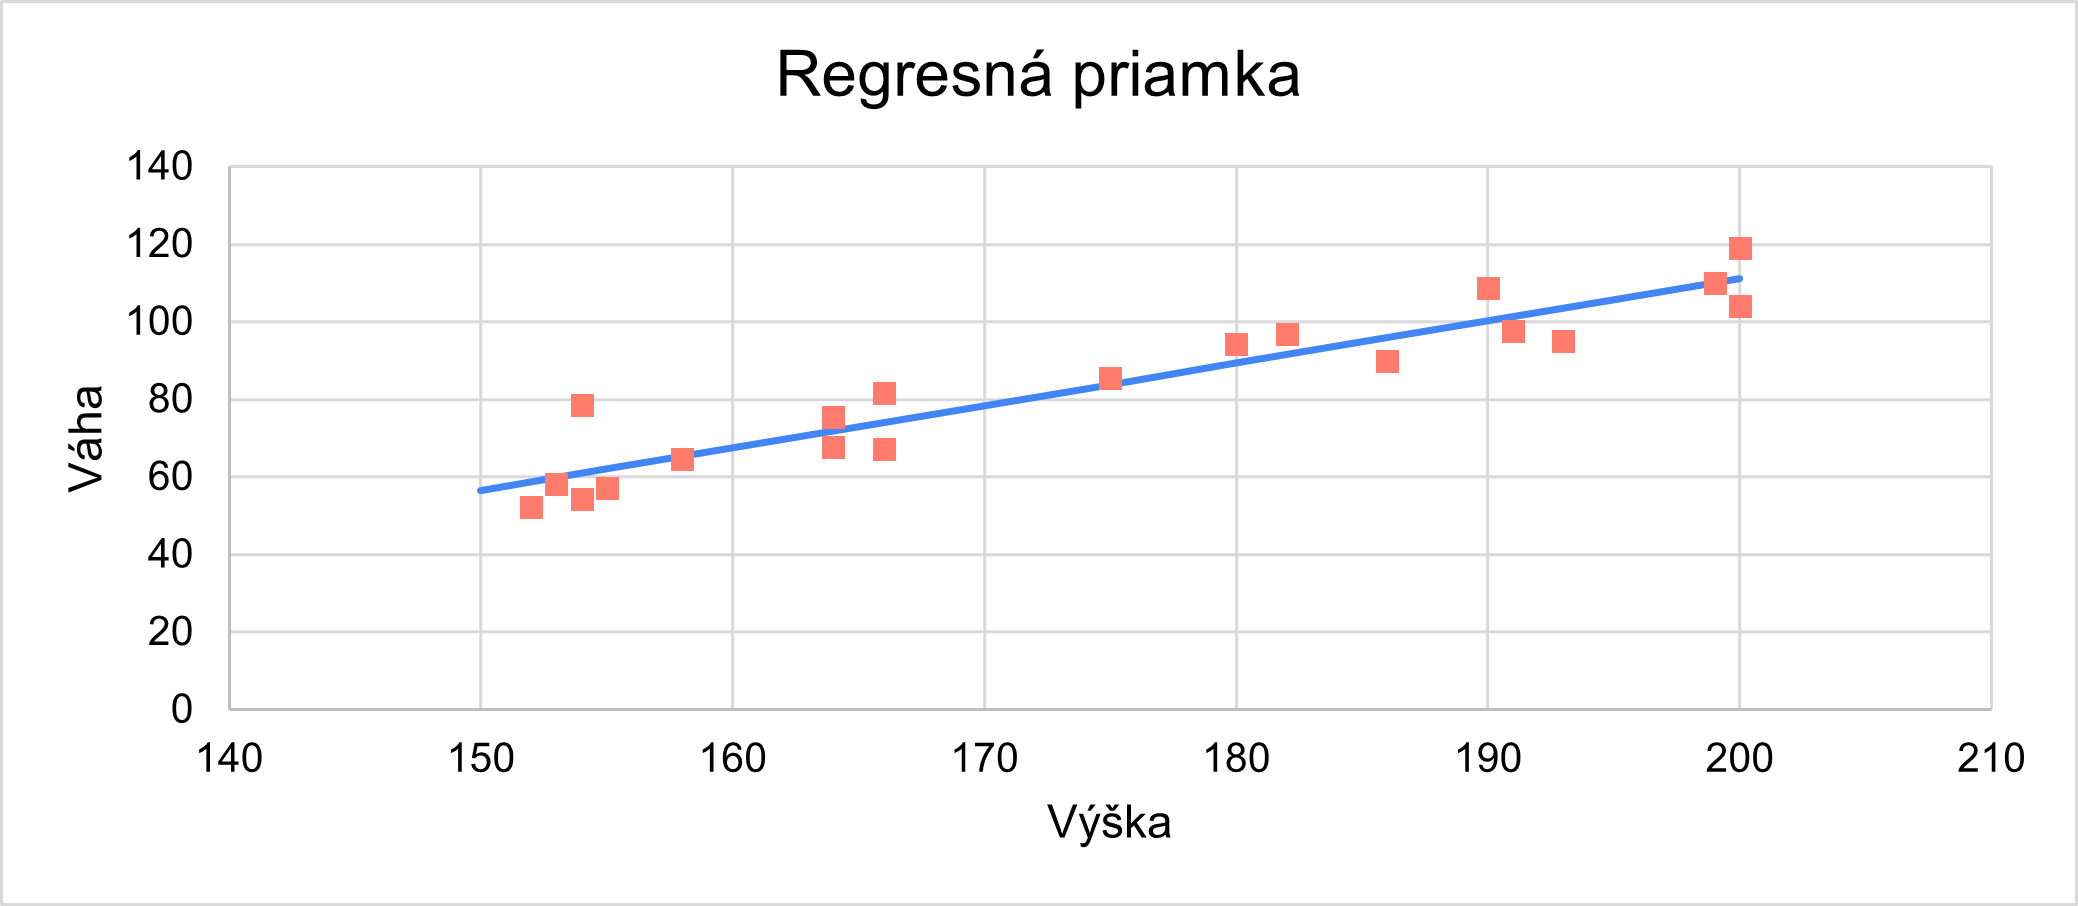
\includegraphics[scale=0.85]{regresna_priamka.png}\\
    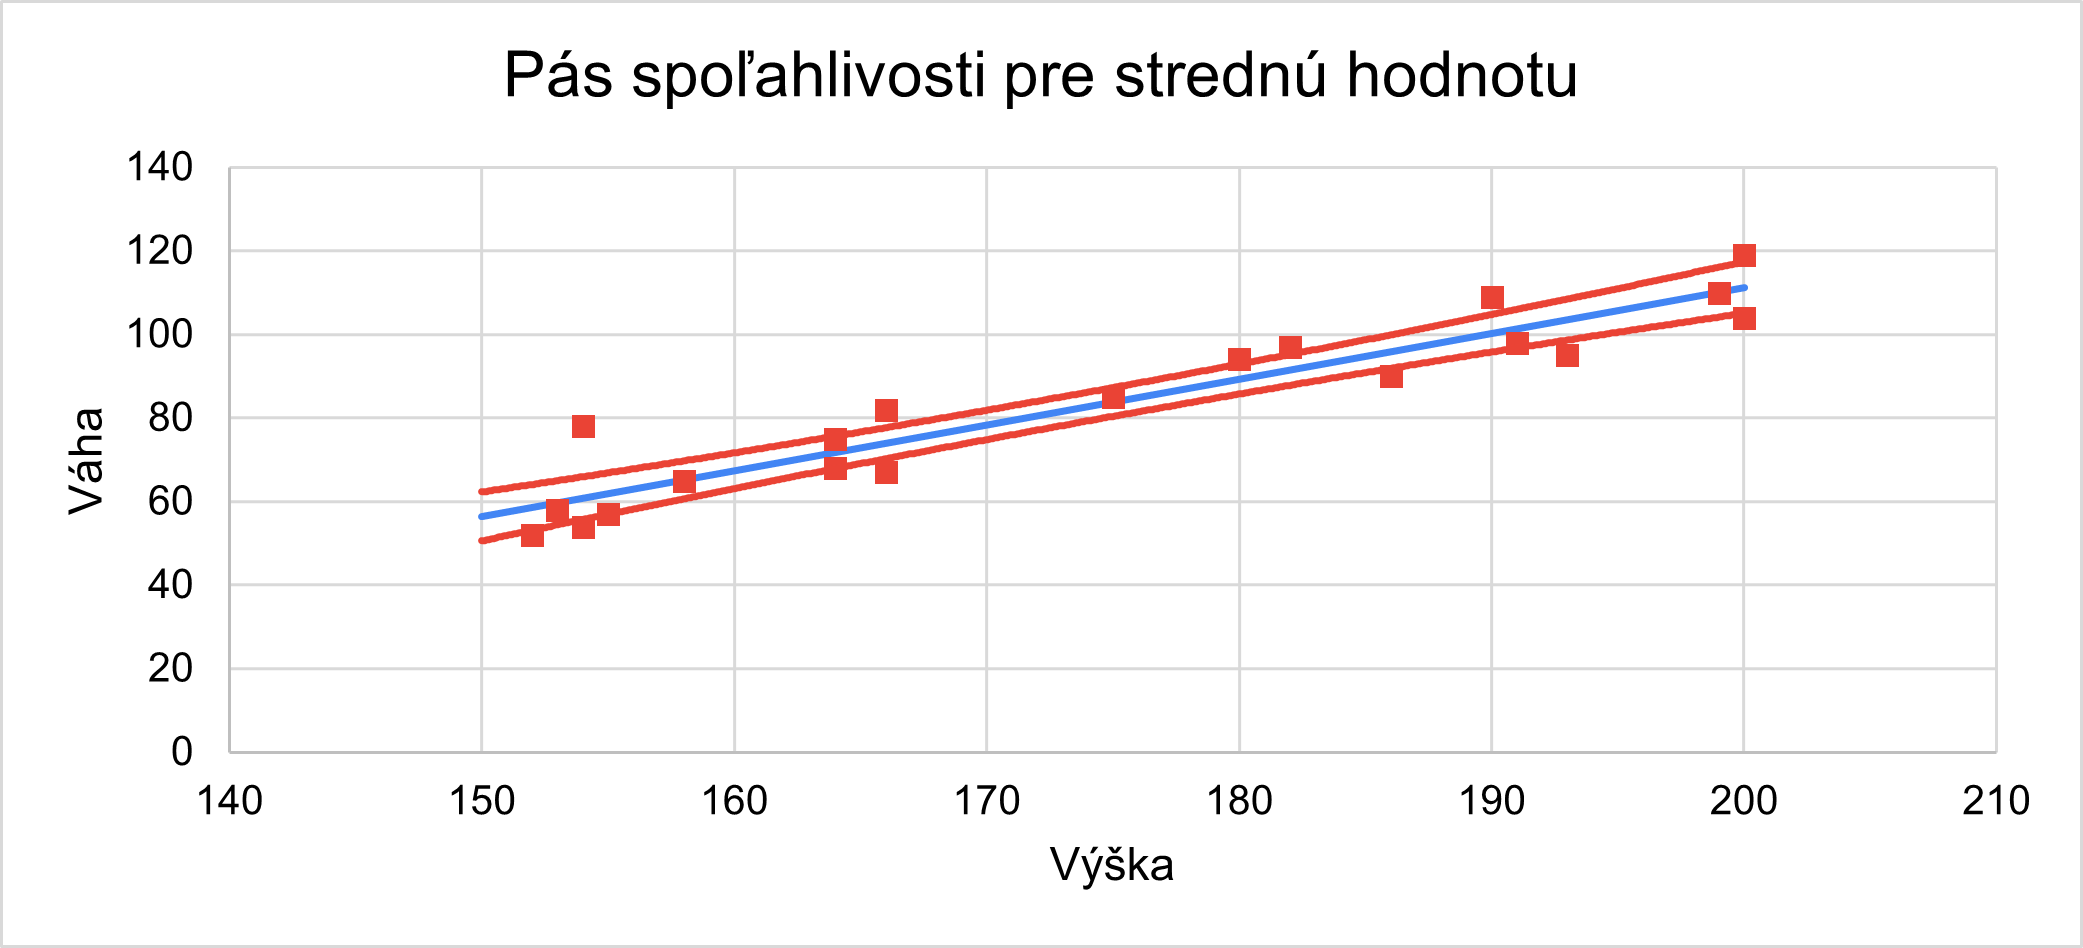
\includegraphics[scale=0.85]{pas_spolahl_pre_strednu_hodnotu.png}\\
    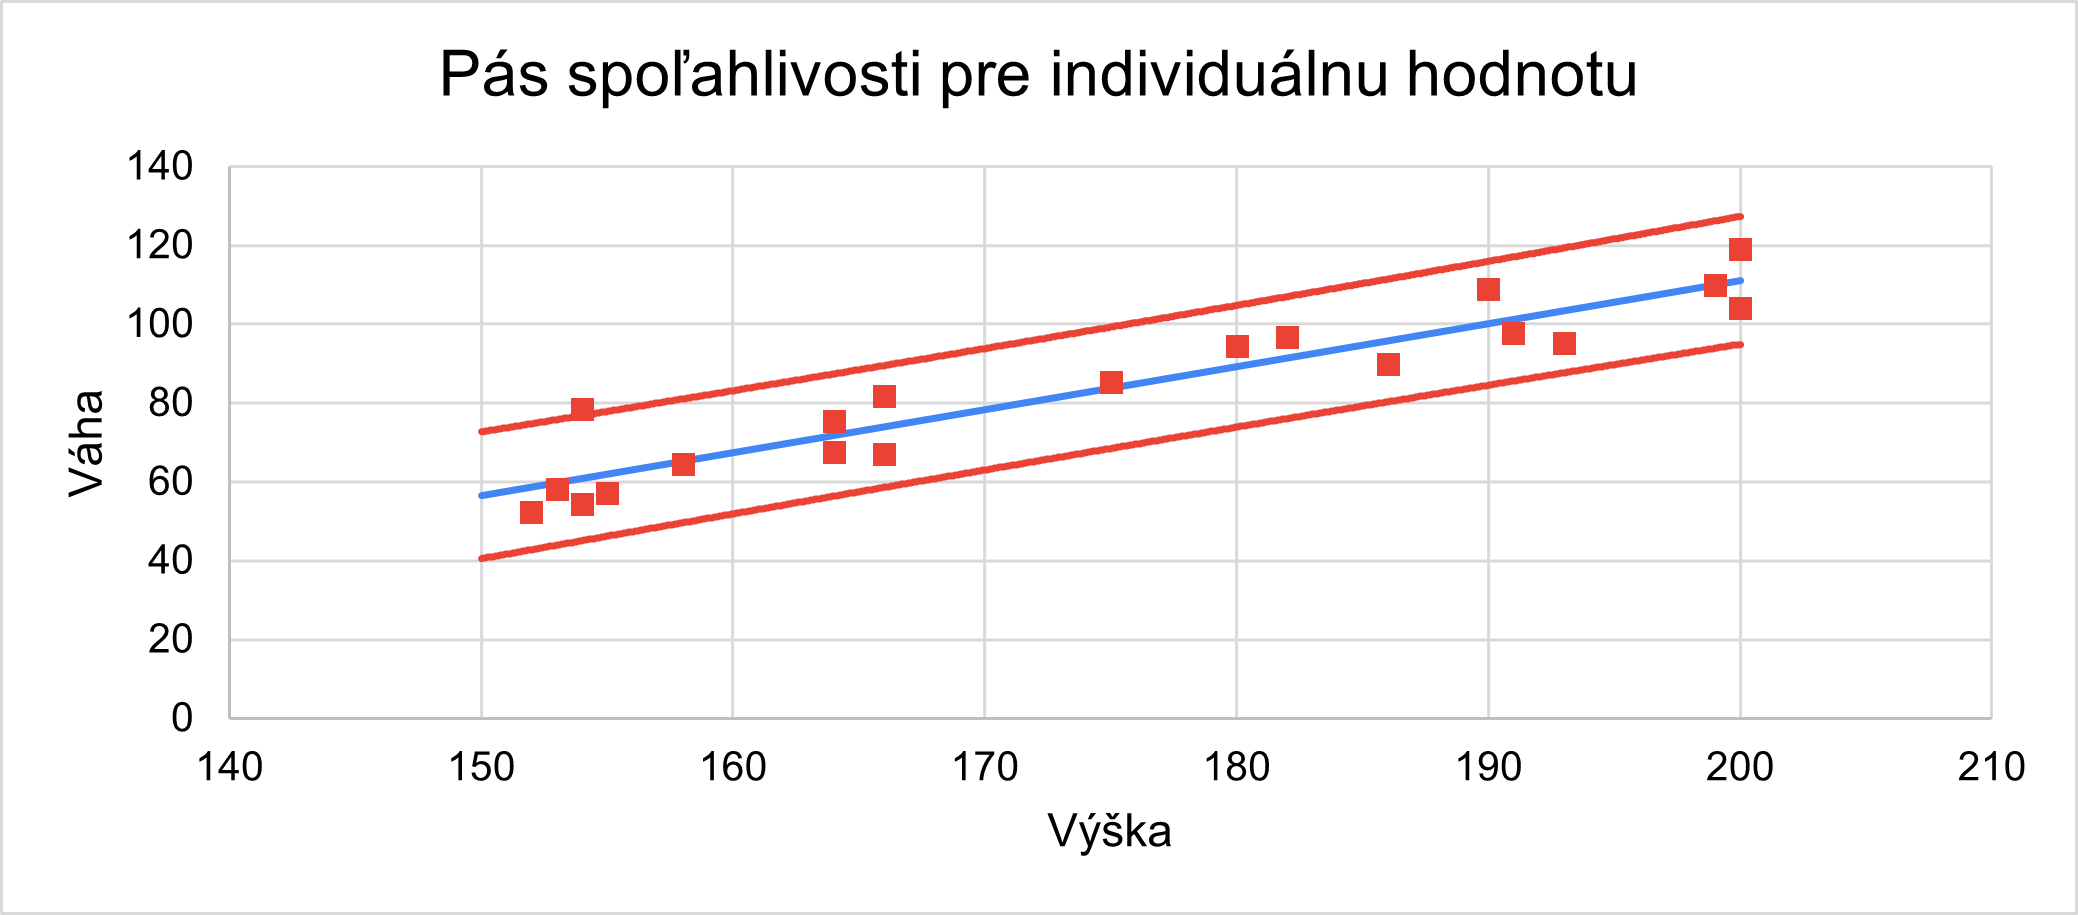
\includegraphics[scale=0.85]{pas_spolahl_pre_individualnu_hodnotu.png}\\
\end{document}
